\documentclass[11pt,letterpaper]{article}

\usepackage[margin=1in]{geometry}
\usepackage{amsmath,amssymb}
\usepackage{mathtools}
\usepackage{booktabs}
\usepackage{enumitem}
\usepackage{hyperref}
\usepackage[dvipsnames]{xcolor}
\usepackage{titlesec}
\usepackage{microtype}
\usepackage{parskip}
\usepackage{array}
\usepackage{tikz}
\usetikzlibrary{arrows.meta,positioning}

\hypersetup{
  colorlinks=true,
  linkcolor=NavyBlue,
  citecolor=NavyBlue,
  urlcolor=NavyBlue,
  pdfstartview=FitH
}

\titleformat{\section}{\large\bfseries}{\thesection}{1em}{}
\titleformat{\subsection}{\normalsize\bfseries}{\thesubsection}{1em}{}
\titleformat{\subsubsection}{\normalsize\itshape}{\thesubsubsection}{1em}{}

\newcommand{\bfp}{\mathbf{p}}
\newcommand{\bfu}{\mathbf{u}}
\newcommand{\bfg}{\mathbf{g}}
\newcommand{\bfh}{\mathbf{h}}
\newcommand{\bfs}{\mathbf{s}}
\newcommand{\bfv}{\mathbf{v}}
\newcommand{\bfz}{\mathbf{z}}
\newcommand{\R}{\mathbb{R}}

\begin{document}

\begin{center}
{\LARGE\bfseries Neural Field Perceiver v14}\\[6pt]
{\large Cross-Patient Speech Decoding via Atlas-Guided Spatial Calibration}\\[10pt]
{\normalsize Ben Tang \quad\textbar\quad Greg Cogan Lab, Duke University}\\[4pt]
{\normalsize April 2026 \quad\textbar\quad Internal architecture spec}
\end{center}

\medskip\noindent\rule{\textwidth}{0.4pt}\medskip

\noindent
Technical design note. This document defines the active v14 architecture only. It does not attempt to be the full SSL spec, experiment program, or paper narrative.


%% ====================================================================
\section{Design Goal}
%% ====================================================================

Each patient's $\mu$ECoG array is a sparse spatial sample of cortical high-gamma activity (HGA, 70--150\,Hz, 200\,Hz) during non-word repetition. Arrays are placed by the surgeon, not by protocol. Across patients, the arrays land on different parts of ventral sensorimotor cortex with different offsets and rotations. Channel indices therefore have no shared meaning.

The architecture must solve one concrete problem: map variable electrode layouts into a common representation that can support one shared phoneme decoder. The output target is a 3-phoneme sequence over 9 phoneme classes for each trial. The input window is full-trial HGA, default $t_{\min}=-0.2$\,s to $t_{\max}=1.0$\,s relative to response onset~\cite{duraivel2023}.

\textbf{Design target:} produce a patient-independent regional representation that preserves speech-relevant structure well enough for one shared dynamical decoder to operate across patients. Before parcellation, that structure is geometric. After parcellation, it is primarily relational: a small graph of atlas-defined regions with learned temporal dynamics.


%% ====================================================================
\section{Core Decomposition}
%% ====================================================================

v14 is organized around a hard boundary between two subproblems:

\begin{enumerate}[leftmargin=2em, itemsep=0.15em]
\item \textbf{Spatial calibration} (per-patient, physics-constrained): electrodes $\to$ atlas-grounded regional tokens.
\item \textbf{Shared dynamics} (shared, unconstrained ML): atlas-grounded regional tokens $\to$ phoneme sequence through a small relational dynamical model.
\end{enumerate}

The interface tensor is
\begin{equation}
\bfz \in \R^{N_{\text{tok}} \times d \times T},
\end{equation}
with default $N_{\text{tok}}=21$, feature dimension $d$, and downsampled time axis $T$.

The default common space uses 16 base Brainnetome parcels but does \emph{not} force one token per parcel. Instead, a small shared within-parcel Perceiver-style summarizer emits a fixed number $K_l$ of atlas/subparcel tokens per parcel. The default token count allocates multiple summaries only where single-token collapse is most likely to over-compress somatotopy:
\begin{itemize}[leftmargin=2em, itemsep=0.15em]
\item 2 tokens each for \textbf{A6cvl, A4hf, A1/2/3ulhf, A2, A1/2/3tonIa}
\item 1 token each for the remaining 11 parcels
\end{itemize}
for a default total of 21 regional tokens. \textbf{A4tl} is the first additional split candidate and raises the interface to 22 tokens when enabled.

Everything before this tensor is calibration: it defines where each patient's measurements land in a common anatomical frame. Everything after this tensor is shared dynamics: it defines what those aligned signals mean for speech decoding.

This is \textbf{not} framed as multi-view reconstruction. There is no reprojection loss, no simultaneous observation from multiple views, and no epipolar structure to recover. The atlas provides the dominant spatial prior; learned per-patient parameters make bounded corrections to that prior.


%% ====================================================================
\section{Model Overview}
%% ====================================================================

\begin{center}
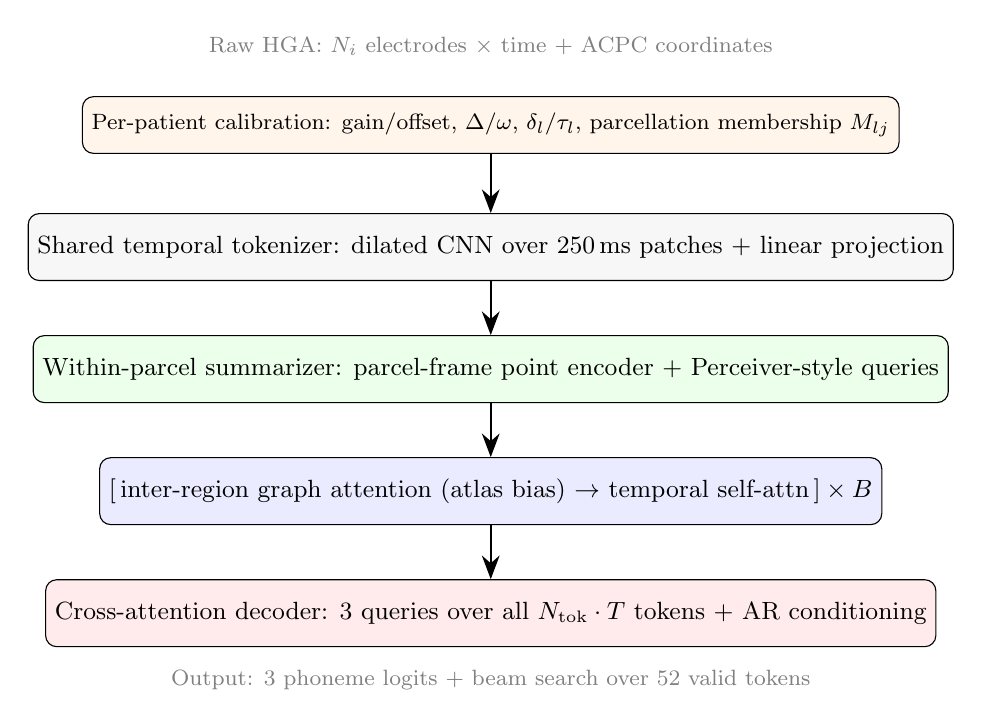
\begin{tikzpicture}[
  box/.style={draw, rounded corners, minimum width=7.1cm, minimum height=0.85cm, align=center, font=\small},
  smallbox/.style={draw, rounded corners, minimum width=7.1cm, minimum height=0.72cm, align=center, font=\footnotesize},
  arrow/.style={-{Stealth[length=3mm]}, thick}
]

\node[smallbox, fill=orange!8] (calib) at (0, 3.7) {Per-patient calibration: gain/offset, $\Delta/\omega$, $\delta_l/\tau_l$, parcellation membership $M_{lj}$};
\node[box, fill=gray!6] (conv) at (0, 2.15) {Shared temporal tokenizer: dilated CNN over 250\,ms patches + linear projection};
\node[box, fill=green!8] (pool) at (0, 0.6) {Within-parcel summarizer: parcel-frame point encoder + Perceiver-style queries};
\node[box, fill=blue!8] (blocks) at (0, -0.95) {$[\,$inter-region graph attention (atlas bias) $\to$ temporal self-attn$\,] \times B$};
\node[box, fill=red!8] (dec) at (0, -2.5) {Cross-attention decoder: 3 queries over all $N_{\text{tok}} \cdot T$ tokens + AR conditioning};

\draw[arrow] (calib) -- (conv);
\draw[arrow] (conv) -- (pool);
\draw[arrow] (pool) -- (blocks);
\draw[arrow] (blocks) -- (dec);

\node[font=\footnotesize, text=gray] at (0, 4.7) {Raw HGA: $N_i$ electrodes $\times$ time + ACPC coordinates};
\node[font=\footnotesize, text=gray] at (0, -3.35) {Output: 3 phoneme logits + beam search over 52 valid tokens};
\end{tikzpicture}
\end{center}

Data flow is simple. Raw HGA is first calibrated in signal space and coordinate space. Each patient's electrodes are then mapped into the same atlas-grounded token space using Brainnetome parcellation membership plus a small shared within-parcel Perceiver-style summarizer in canonical parcel coordinates. At that point the representation is no longer a Euclidean sensor layout; it is a small set of atlas tokens linked by anatomical and functional relations. A shared relational-temporal backbone contextualizes those tokens, and a small cross-attention decoder reads out the 3-phoneme sequence.

\begin{table}[ht!]\centering\small
\begin{tabular}{@{}lrll@{}}
\toprule
\textbf{Module} & \textbf{Params} & \textbf{Shared?} & \textbf{Role} \\
\midrule
Temporal tokenizer (dilated CNN + projection) & ${\sim}$5--8K & Shared & Per-channel temporal feature extraction \\
Point encoder + local Perceiver summarizer & ${\sim}$8--15K & Shared & Local parcel-field estimation \\
Relational-temporal blocks ($B=2$) & ${\sim}$130K & Shared & Atlas-token graph dynamics \\
Cross-attention decoder & ${\sim}$13K & Shared & Joint space-time readout over $N_{\text{tok}} \cdot T$ \\
\midrule
Gain + offset & $2N_{\text{ch}}$/pt & Per-patient & Signal calibration \\
$\Delta + \omega$ & 6/pt & Per-patient & Global registration correction \\
$\delta_l$ & 48/pt & Per-patient & Per-region offsets \\
$\tau_l$ & 16/pt & Per-patient & Per-region sharpness \\
\midrule
\textbf{Total shared} & $\mathbf{{\sim}156\text{--}166}$\textbf{K} & & \\
\textbf{Per-patient (128-ch)} & \textbf{326} & & $2N_{\text{ch}} + 70$ \\
\bottomrule
\end{tabular}
\end{table}


%% ====================================================================
\section{Spatial Calibration}
%% ====================================================================

\subsection{Signal calibration}

Each channel receives a per-patient gain and offset before any shared nonlinearity:
\begin{equation}
\hat{x}_j(t) = \operatorname{softplus}(s_j^{(i)}) \cdot x_j(t) + b_j^{(i)}.
\end{equation}

This is diagonal normalization, not a learned affine mixing across channels. The intent is simple: compensate for gain and baseline differences so that the shared temporal tokenizer sees comparable amplitudes across patients. Applying this before the nonlinear temporal encoder is deliberate; after the nonlinearity the ordering is no longer equivalent.

\subsection{Coordinate correction}

Electrode coordinates start in ACPC space, pass through the patient's fixed talairach affine, then receive a learned rigid correction:
\begin{equation}
\tilde{\bfp}_j = R(\omega^{(i)}) \bigl(T_{\text{xfm}}^{(i)} \bfp_j^{\text{ACPC}}\bigr) + \Delta^{(i)}.
\end{equation}

$\Delta^{(i)}$ and $\omega^{(i)}$ absorb global residual error from surgical reconstruction and linear-only MNI normalization. They are hard-clamped and regularized because they are meant to fix coarse global misregistration, not to learn patient-specific anatomy from scratch.

\subsection{Region adaptation and membership}

The common spatial frame starts from a fixed set of 16 Brainnetome parcels chosen for speech relevance and patient reachability: 3 motor, 3 sensory, 6 Broca's, 2 auditory, 1 insular, and 1 executive region~\cite{fan2016,glasser2016}. Each parcel has a small patient-specific offset and a scalar temperature:
\begin{equation}
\bfp_l^{(i)} = \bfp_l^{\text{atlas}} + \delta_l^{(i)}, \qquad \tau_l^{(i)} \in [0.3, 3.0].
\end{equation}

Region membership is read from volumetric Brainnetome maps rather than spherical kernels:
\begin{equation}
M_{lj} = \operatorname{interp}\!\left(\text{atlas\_prob}_l(\cdot - \delta_l^{(i)}),\; \tilde{\bfp}_j\right)^{1/\tau_l^{(i)}}.
\end{equation}

This is the core spatial choice in v14. The model does not learn where a parcel is by content-based routing. It starts from the atlas, adjusts each parcel locally, and uses soft volumetric membership to map electrodes into a common anatomical frame. The result is a calibration mechanism, not an electrode-to-region attention module.

\subsection{Default token counts}

Single-token-per-parcel collapse is not the default. Several speech-relevant strip parcels are too elongated for one token to carry both activation magnitude and within-parcel location without excessive compression. The default sub-token count map is
\begin{equation}
S_l =
\begin{cases}
2, & l \in \{\text{A6cvl, A4hf, A1/2/3ulhf, A2, A1/2/3tonIa}\}, \\
1, & \text{otherwise},
\end{cases}
\qquad
N_{\text{tok}} = \sum_l S_l = 21.
\end{equation}

This keeps the atlas prior fixed while allowing large parcels to emit multiple tokens only where the geometry strongly suggests that single-token collapse is too coarse. \textbf{A4tl} is intentionally left as the first extension candidate rather than a default split; enabling it raises the interface to 22 tokens and remains an explicit ablation.

\subsection{Default within-parcel Perceiver summarizer}

Precision-style $\mu$ECoG suggests that the true local cortical field is richer than a single parcel mean plus one first spatial moment: adjacent contacts remain incompletely correlated at sub-millimetre spacing, especially in high gamma. Combined with the recent realization that some speech decoding may be dominated by a small number of locally informative parcels, this is enough to promote a local summarizer to the default spatial interface. The important constraint is still identifiability: our practical alignment floor remains on the order of 5--15\,mm and parcel coverage is often sparse and asymmetric across patients, so the summarizer must stay small, shared, and anatomically anchored rather than becoming a free-form routing module.

v14 therefore preserves atlas-grounded calibration but inserts a small \emph{shared local Perceiver-style summarizer} inside each parcel before final token collapse. For electrode $j$ in parcel $l$, define canonical parcel-frame coordinates
\begin{equation}
\bfu_{lj} = A_l^{-1} R_l^\top \bigl(\tilde{\bfp}_j - \bfp_l^{(i)}\bigr) \in \R^3,
\end{equation}
where $R_l$ aligns the atlas parcel to its principal axes and $A_l$ rescales by parcel axis lengths. This expresses local geometry in a parcel-normalized frame rather than raw global coordinates.

The local point-encoder input is
\begin{equation}
\bfg_{lj}(t) = \bigl[f_j(t);\; \bfu_{lj};\; M_{lj};\; c_{lj}\bigr],
\end{equation}
where $c_{lj}$ is an optional support/confidence signal. A shared point encoder
\begin{equation}
\bfh_{lj}(t) = E_{\mathrm{local}}\!\bigl(\bfg_{lj}(t), e_l\bigr)
\end{equation}
maps those inputs to a local latent, with $e_l$ a small parcel embedding or parcel-group adapter. The weights of $E_{\mathrm{local}}$ are shared across patients and parcels; only the lightweight conditioning varies. This is the important rigidity constraint: local flexibility without a separate learned geometry module per patient or per parcel.

Each parcel then emits $K_l$ local summaries through fixed-count latent queries that cross-attend to the local set:
\begin{equation}
\alpha_{lkj}(t) = \operatorname{Softmax}_j\!\left(q_{lk}^\top \bfh_{lj}(t) + \log(M_{lj} + \epsilon)\right),
\qquad
\bfs_{lk}(t) = \sum_j \alpha_{lkj}(t)\, \bfh_{lj}(t),
\end{equation}
for $k=1,\dots,K_l$, with $K_l$ typically 1--3 depending on parcel size and support. This is deliberately a \emph{local} cross-attention mechanism: atlas membership already determines which electrodes belong to parcel $l$, and the learned queries only summarize the parcel-conditioned local set. These $\bfs_{lk}(t)$ sub-tokens replace the single pooled token for parcel $l$ while still landing in the same atlas/subparcel token space used by the shared backbone.

This is now the default hierarchy:
\begin{enumerate}[leftmargin=2em, itemsep=0.15em]
\item \textbf{Local Perceiver-style summarizer:} encode parcel-frame points and summarize them with fixed-count latent queries.
\item \textbf{Atlas/subparcel tokens:} collapse local structure into a fixed, comparable token interface.
\item \textbf{Shared dynamics:} model speech-relevant temporal and inter-parcel interactions after spatial alignment.
\end{enumerate}

Two simpler special cases sit inside this same template. \textbf{Selective parcel splitting} is the hand-designed two-state version. \textbf{Mean+gradient pooling} is the linear first-order version and remains the main simplifying ablation. A tiny \textbf{2D conv local encoder} is also possible when electrodes densely sample a cortical sheet: project parcel-frame coordinates to a local tangent plane, rasterize a small patch, and apply Conv2d. That is not the default because it is brittle under sparse irregular coverage and does not transfer naturally to sEEG. The key distinction from the rejected global routing variant is scope: the Perceiver-style cross-attention happens \emph{within a parcel after atlas assignment}, not across all electrodes and all regions.


%% ====================================================================
\section{Shared Dynamics}
%% ====================================================================

\subsection{Temporal tokenization}

Instead of a minimal Conv1d downsampling stem, v14 now adopts a \textbf{BaRISTA-style shared temporal tokenizer}. Each calibrated electrode trace is divided into overlapping temporal patches
\begin{equation}
P_{jr} = \hat{x}_j[t_r:t_r+L-1], \qquad L = 250\,\text{ms},
\end{equation}
with stride 50\,ms so the downstream time axis remains at 20\,Hz. Each patch is passed through a shared dilated temporal encoder and projected into the model dimension:
\begin{equation}
f_j(r) = W_{\mathrm{tok}}\, E_{\mathrm{temp}}(P_{jr}) \in \R^d.
\end{equation}

This stage is shared across all electrodes and patients. Its job is no longer just temporal binning; it extracts a richer local oscillatory representation before any atlas pooling occurs. This imports the strongest low-level idea from BaRISTA without adopting its global channel-token architecture. Continuous geometry still enters only at the atlas-grounded pooling stage.

\subsection{Atlas-token formation}

The default atlas-token tensor passed to the shared backbone is assembled from the local summaries $\bfs_{lk}(t)$ produced by the within-parcel Perceiver summarizer above. In other words, the token for atlas/subparcel state $(l,k)$ is
\begin{equation}
\bfz_m(t) = \bfs_{lk}(t), \qquad m \leftrightarrow (l,k).
\end{equation}

The old linear pooling rule is kept as the primary ablation. Let $l(m)$ denote the parent parcel of token $m$. For a token $m$ with gating weights $G_{mj}$, the token mean is
\begin{equation}
\bfz_m^{\text{mean}} = \frac{\sum_j G_{mj} f_j}{\sum_j G_{mj}}.
\end{equation}

Its first-order spatial term uses the electrode offset from the parent parcel center:
\begin{equation}
\bfz_m^{\text{grad}} = \frac{\sum_j G_{mj}\, \bigl(f_j \odot W_{\text{pos}}(\tilde{\bfp}_j - \bfp_{l(m)}^{(i)})\bigr)}{\sum_j G_{mj}},
\qquad W_{\text{pos}} \in \R^{d \times 3}.
\end{equation}

The resulting linear token representation is
\begin{equation}
\bfz_m = \bfz_m^{\text{mean}} + \bfz_m^{\text{grad}}.
\end{equation}

This linear rule remains useful precisely because it is the simplest way to test whether the default local Perceiver summarizer is buying real signal rather than just extra capacity. Cross-attention remains a separate ablation because electrode-to-region mapping is still being treated as anatomy-guided aggregation, not unconstrained content routing.

\subsection{Relational-temporal backbone}

After pooling, the model operates on $N_{\text{tok}} \times T$ atlas-grounded tokens. This is the regime change in v14: before pooling, the model lives in continuous electrode geometry; after pooling, it lives in a small relational token space. Each block alternates:

\begin{enumerate}[leftmargin=2em, itemsep=0.15em]
\item \textbf{Inter-region graph attention} across the $N_{\text{tok}}$ atlas tokens at each time step.
\item \textbf{Temporal self-attention} within each atlas token across time.
\end{enumerate}

The inter-region attention bias is initialized from Brainnetome structural and functional connectivity. Split tokens inherit the bias of their parent parcel, optionally with a small within-parcel attraction bias between sibling tokens. This is a small-data prior: the model should not have to learn a token interaction graph from scratch when the atlas already encodes a plausible Broca's-to-motor-to-sensory-to-auditory cascade.

Temporal dynamics remain shared by default. If mild specialization is needed, the next step is parcel or parcel-group conditioning inside the shared temporal blocks, not a fully separate temporal encoder per parcel. Fully distinct temporal stacks are deferred because they reduce data efficiency and weaken the common latent space that the atlas interface is supposed to create.

\subsection{Decoder}

Three learned phoneme-position queries attend jointly to all atlas-token time tokens:
\begin{equation}
q_k' = q_k + \operatorname{emb}(y_{k-1}), \qquad
o_k = \operatorname{CrossAttn}(q_k', \text{KV} = N_{\text{tok}} \cdot T \text{ tokens}), \qquad
\hat{y}_k = \operatorname{Linear}(o_k).
\end{equation}

This replaces the older temporal-pooling readout. The decoder is allowed to read any region at any time for any phoneme position. That is the point: phoneme 3 may need early Broca's planning and late motor execution, and a rigid pooled slot is too restrictive.


%% ====================================================================
\section{Training Assumptions}
%% ====================================================================

\subsection{Staged optimization}

Training follows the same boundary as the architecture:

\begin{enumerate}[leftmargin=2em, itemsep=0.15em]
\item \textbf{Stage 1:} train shared dynamics with only coarse geometric correction active ($\Delta/\omega$).
\item \textbf{Stage 2:} unfreeze per-region offsets and temperatures ($\delta_l, \tau_l$).
\item \textbf{Stage 3:} end-to-end fine-tuning.
\end{enumerate}

This is not a claim about optimal optimization in general. It is a practical way to separate global registration from region-level refinement and avoid asking the smallest, most weakly identified parameters to solve the whole problem immediately.

\subsection{Default supervised objective}

The default loss is
\begin{equation}
\mathcal{L}
=
\sum_i w^{(i)} \frac{1}{3}\sum_{k=1}^{3} \operatorname{FocalCE}(\hat{y}_k, y_k)
+ \lambda_{\Delta\omega} E_{\Delta\omega}
+ \lambda_{\delta} E_{\delta}
+ \lambda_{\text{sm}} E_{\text{smooth}}.
\end{equation}

$E_{\Delta\omega}$ regularizes global coordinate correction, $E_{\delta}$ regularizes per-region deformation, and $E_{\text{smooth}}$ regularizes regional temporal trajectories. Standard dropout, DropPath, channel dropout, and AdamW remain part of the default recipe, but they are secondary to the architectural split above.

\subsection{SSL note}

Default SSL is JEPA-style temporal masking. In v14, SSL is intended to pretrain the shared temporal and dynamical stack, not the spatial calibration mechanism. The working assumption is that atlas-guided calibration dominates the spatial problem, while SSL mainly improves the quality of the shared regional dynamics model.


%% ====================================================================
\section{Ablations}
%% ====================================================================

The main ablations should directly test the architectural claims and the main failure modes: partial atlas coverage, over-compression into too few regions, weakly identified geometry, decoder over-capacity, and SSL objectives that accidentally train on unobserved parcels.

\subsection{Priority architectural ablations}

\begin{table}[ht!]\centering\small
\begin{tabular}{@{}>{\raggedright\arraybackslash}p{2.9cm}>{\raggedright\arraybackslash}p{2.9cm}>{\raggedright\arraybackslash}p{3.1cm}>{\raggedright\arraybackslash}p{5.0cm}@{}}
\toprule
\textbf{Question} & \textbf{Default mechanism} & \textbf{Key ablation(s)} & \textbf{What the result would mean} \\
\midrule
Is missing parcel coverage handled correctly? & Coverage-aware regional tokens with explicit support/confidence mask; unobserved parcels excluded from losses and normalization & Coverage-aware vs coverage-naive (treat low-support parcels as zeros) & If coverage-aware wins, the model was previously conflating ``missing'' with ``observed but quiet.'' This becomes a core part of the spatial interface, not an implementation detail. \\
Is the default tokenization still too coarse? & 21-token default from 16 Brainnetome parcels via shared within-parcel Perceiver summarizer with $K_l \in \{1,2\}$ & 16 unsplit vs 21 default vs 22 with A4tl split vs 24-token variants & If 16 unsplit matches default, multi-token parcel summaries are unnecessary. If 22 or 24 wins, the default is still over-compressing speech-relevant spatial structure, especially within elongated motor/sensory parcels. \\
Is electrode-to-region mapping calibration rather than content routing? & Atlas-guided local aggregation with fixed membership & Region cross-attention; distance/RBF pooling baseline & If routing wins clearly, the spatial stage needs more learned flexibility than assumed. If local aggregation holds, the calibration framing is correct. \\
Is a nonlinear local summarizer actually needed? & Shared within-parcel Perceiver summarizer & Mean + gradient pooling; mean-only pooling & If mean+gradient matches default, the nonlinear local stage is unnecessary in this regime. If mean-only also holds up, even first-order local structure is not carrying useful cross-patient information. \\
What is the right local summarizer class? & Shared within-parcel Perceiver summarizer & Parcel-frame 2D local Conv for dense surface data; low-rank basis pooling & If the Perceiver summarizer wins broadly, irregular-geometry set summarization matters more than grid-specific locality. If 2D Conv wins on dense surface data only, keep it as a modality-specific variant rather than the common default. \\
Do patients need staged calibration? & Stage 1 $\Delta/\omega$ only, then $\delta_l,\tau_l$, then end-to-end & Staged optimization vs full joint training from step 1 & If staged training wins, weakly identified spatial parameters need a calibration curriculum rather than fully joint optimization. \\
Which geometric refinements actually matter? & Full geometry refinement: $\Delta/\omega + \delta_l + \tau_l$ & Fixed coordinates; rigid only; rigid + $\delta_l$; rigid + $\delta_l + \tau_l$ & This isolates whether gains come from coarse registration, local region shifts, or region sharpness. It also tests whether the per-region deformation budget is justified. \\
\bottomrule
\end{tabular}
\end{table}

\begin{table}[ht!]\centering\small
\begin{tabular}{@{}>{\raggedright\arraybackslash}p{2.9cm}>{\raggedright\arraybackslash}p{2.9cm}>{\raggedright\arraybackslash}p{3.1cm}>{\raggedright\arraybackslash}p{5.0cm}@{}}
\toprule
\textbf{Question} & \textbf{Default mechanism} & \textbf{Key ablation(s)} & \textbf{What the result would mean} \\
\midrule
Does atlas interaction structure help? & Inter-region graph attention with atlas SC/FC bias init & Random bias init; no bias term & If random or no-bias matches default, the connectivity prior is cosmetic. If default helps, the atlas is carrying useful region-interaction structure. \\
Should temporal dynamics stay fully shared across parcels? & Shared temporal blocks with parcel identity only through the token interface & Parcel-group adapters; fully distinct temporal encoders per parcel & If parcel-group conditioning helps, some specialization is useful without giving up comparability. If fully separate temporal encoders win clearly, the shared dynamics hypothesis is weaker than assumed. \\
Is the flexible decoder actually necessary? & Cross-attention decoder over all $N_{\text{tok}} \cdot T$ tokens with AR conditioning & Temporal pooling + linear head; cross-attention without AR conditioning & If pooled readout matches default, the decoder is overbuilt. If AR removal hurts but cross-attention remains strong, autoregressive conditioning is doing real work rather than just the joint readout. \\
Can the shared model tolerate partial observability? & Coverage-aware training plus region/electrode dropout augmentation & Coverage robustness: with vs without synthetic electrode subset dropout and synthetic parcel dropout; evaluate under reduced test-time coverage & If robustness training helps, the common-space decoder needs explicit exposure to the coverage patterns it will face across patients. \\
\bottomrule
\end{tabular}
\end{table}

\subsection{Priority SSL ablations}

\begin{table}[ht!]\centering\small
\begin{tabular}{@{}>{\raggedright\arraybackslash}p{2.9cm}>{\raggedright\arraybackslash}p{2.9cm}>{\raggedright\arraybackslash}p{3.1cm}>{\raggedright\arraybackslash}p{5.0cm}@{}}
\toprule
\textbf{Question} & \textbf{Default mechanism} & \textbf{Key ablation(s)} & \textbf{What the result would mean} \\
\midrule
Should JEPA see missing parcels as targets? & Mask-aware JEPA: only visible parcel-time targets contribute to the SSL loss & Mask-aware JEPA vs naive JEPA over all parcels & If mask-aware wins, the naive objective was forcing the model to hallucinate dynamics in unobserved parcels. \\
Does robustness require parcel-level dropout in SSL? & JEPA with region/electrode dropout augmentation & Region dropout in SSL vs none & If dropout helps, the SSL objective benefits from learning under partial atlas support rather than only under full observed coverage. \\
Does JEPA help at all in this regime? & JEPA pretraining followed by supervised fine-tuning & JEPA vs no pretraining & This is the fundamental SSL sanity check. Without it, the pretraining story is not established. \\
What target granularity should JEPA use? & Visible-target parcel-time prediction & Visible targets only vs dense prediction over all visible+unmasked tokens & If dense prediction helps, extra visible-token supervision stabilizes the backbone. If visible-target-only wins, sparse masked prediction is the cleaner objective. \\
\bottomrule
\end{tabular}
\end{table}

\subsection{Minimal high-priority set if compute is tight}

\begin{enumerate}[leftmargin=2em, itemsep=0.15em]
\item Coverage-aware vs coverage-naive regional tokens.
\item 16 unsplit vs 21 default split vs 22 with A4tl split vs 24-token variants.
\item Within-parcel Perceiver summarizer vs mean+gradient vs mean-only pooling.
\item Staged calibration vs joint training.
\item Full geometry refinement ladder: fixed, rigid only, rigid + $\delta_l$, rigid + $\delta_l + \tau_l$.
\item Cross-attention AR decoder vs pooled decoder vs cross-attention without AR.
\item Atlas connectivity bias init vs random/no bias.
\item Coverage robustness with synthetic parcel/electrode dropout.
\item Mask-aware JEPA vs naive JEPA.
\item Region dropout in SSL.
\item JEPA vs no pretraining.
\item JEPA target granularity: visible-target-only vs dense visible-token prediction.
\end{enumerate}


%% ====================================================================
\section{Open Assumptions and Blockers}
%% ====================================================================

\begin{itemize}[leftmargin=2em, itemsep=0.2em]
\item \textbf{Nonlinear MNI normalization.} The current talairach transform is linear. Residual nonlinear error in the 5--15\,mm range is large enough to matter for any coordinate-based architecture.
\item \textbf{Real probabilistic Brainnetome maps.} The Phase 1 implementation should use the real PM volume at \texttt{/Users/bentang/Documents/Code/speech/data/atlas/BNA\_PM\_4D.nii.gz} as the active membership source. The MPM label map remains useful for ROI indexing and sanity checks only; there should be no silent fallback to the old smoothed-MPM proxy.
\item \textbf{Full-trial input remains an assumption.} The strongest current per-patient result is still per-phoneme MFA. v14 assumes the shared decoder can justify returning to full-trial input, but that is not yet established.
\item \textbf{Several design choices remain claims, not facts.} The within-parcel Perceiver summarizer over its linear pooling ablations, connectivity initialization, and the new decoder all require direct ablation support.
\end{itemize}


\begin{thebibliography}{99}\raggedright

\bibitem{duraivel2023}
Duraivel, S., et al.\ (2023).
High-resolution neural recordings improve the accuracy of speech decoding.
\textit{Nature Communications}, 14, 6938.

\bibitem{roux2020}
Roux, F.-E., et al.\ (2020).
The human motor cortex somatotopy.
\textit{The Journal of Physiology}, 598(23), 5301--5316.

\bibitem{bouchard2013}
Bouchard, K.\,E., Mesgarani, N., Johnson, K., \& Chang, E.\,F.\ (2013).
Functional organization of human sensorimotor cortex for speech articulation.
\textit{Nature}, 495, 327--332.

\bibitem{rademacher2001}
Rademacher, J., et al.\ (2001).
Variability and asymmetry in the human precentral motor system.
\textit{Brain}, 124(11), 2232--2258.

\bibitem{fan2016}
Fan, L., et al.\ (2016).
The Human Brainnetome Atlas.
\textit{Cerebral Cortex}, 26(8), 3508--3526.

\bibitem{glasser2016}
Glasser, M.\,F., et al.\ (2016).
A multi-modal parcellation of human cerebral cortex.
\textit{Nature}, 536, 171--178.

\end{thebibliography}

\end{document}
